\chapter{国际制和高斯制的换算}

这一章讨论电动力学中国际单位和高斯制的换算,目的在于方便的进行相关公式的转换,而在理论物理中常使用的是高斯制,比如量子力学中的电磁场的Sch\"odinger 方程等.其核心考虑为\CJKunderwave{所有的力学量都不改变,仅改变电学量和部分电学量的定义.}

\section{基本公式的转换}

\begin{gather}
  \intertext{电荷的转换,在库仑定律中考虑,可以使比例系数为1,这样表达公式则更方便.国际单位制如下}
  F=\frac{1}{4\pi\varepsilon_0}\frac{q_1q_2}{r^2}
  \intertext{显然,如果使高斯制电荷和国际制的关系为$q'=\frac{q}{\sqrt{4\pi\varepsilon_0}}$,则库仑定律表达为}
  F=\frac{q_1'q_2'}{r^2}
  \intertext{考虑Lorentz 力密度公式}
  \vec{f}=q\vec{E}+q\vec{v}\times \vec{B}
  \intertext{由于力的单位不变,所以应当有}
  q\vec{E}=q'\vec{E}'
  \intertext{因此得电场强度的变换为$\vec{E}'=\sqrt{4\pi\varepsilon_0}\vec{E}$,同时再来考虑磁感应强度,在国际单位制中电场强度和磁感应强度的比为光速,即$\frac{E}{B}=c$,但是电场和磁场是同一种物质的不同方面,所以这是不协调的.所以在高斯制中统一使磁感应强度扩大$c$倍,这样新定义的磁感应强度和电场强度就是同一数量级了.如下}
  q\vec{v}\times\vec{B}=q'\frac{\vec{v}}{c}\times \sqrt{4\pi\varepsilon_0}c\vec{B}=q'\frac{\vec{v}}{c}\times \vec{B}'
  \intertext{于是得磁感应强度的转换关系为$\vec{B}'=\sqrt{4\pi\varepsilon_0}c\vec{B}$.下面再来考虑电势和磁矢势的改变,由于$\vec{E}=-\nabla \varphi$,而力学量不变,则电势和电场强度的变换是相同的,即$\varphi'=\sqrt{4\pi\varepsilon_0}\varphi$,同时由$\vec{B}=\nabla\times\vec{A}$可知,$\vec{A}$和$\vec{B}$的变换规则相同,即$\vec{A}'=\sqrt{4\pi\varepsilon_0}c\vec{A}$,下面讨论 Maxwell 方程的变换.第一式,法拉第电磁感应定律国际制为}
  \nabla\times\vec{E}=-\frac{\partial\vec{B}}{\partial t}  
  \intertext{对于上式可以同时乘以$\sqrt{4\pi\varepsilon_0}$再对右式分子分母同时乘以$c$,也可以根据修改后的$\vec{E}$和$\vec{B}$同量级来写出高斯制的方程为}
  \nabla\times\vec{E}'=-\frac{1}{c}\frac{\partial\vec{B}'}{\partial t}  
  \intertext{下面考虑 Maxwell 第四式,由于其值为0,所以当单位变换时其形式不变,即高斯制下为}
  \nabla\cdot\vec{B}'=0
  \intertext{考虑 Maxwell 第三式,高斯定理的国际制为}
  \nabla\cdot\vec{E}=\frac{\rho}{\varepsilon_0}
  \intertext{上式左右同时乘以$\sqrt{4\pi\varepsilon_0}$得}
  \nabla\cdot\vec{E}'=\sqrt{4\pi\varepsilon_0}\cdot\frac{\sqrt{4\pi\varepsilon_0}\rho'}{\varepsilon_0}
  \intertext{即得 Maxwell 第三式为}
  \nabla\cdot\vec{E}'=4\pi\rho'
  \intertext{下面来考虑 Maxwell 第二式,其国际制为}
  \nabla\times\vec{B}=\mu_0\vec{J}+\frac{1}{c^2}\frac{\partial \vec{E}}{\partial t}
  \intertext{上式同时乘以$\sqrt{4\pi\varepsilon_0}c$考虑到$\vec{J}=\sqrt{4\pi\varepsilon_0}\vec{J}'$则上式化为}
  \nabla\times\vec{B}'=\frac{4\pi}{c}\vec{J}'+\frac{1}{c}\frac{\partial \vec{E}'}{\partial t}
  \intertext{下面我们罗列出由国际制到高斯制的变换关系如下}
  \mbox{\small 基本关系}\quad
  \left\{
    \begin{gathered}
      q'=\frac{q}{\sqrt{4\pi\varepsilon_0}}\\
      \vec{J}'=\frac{\vec{J}}{\sqrt{4\pi\varepsilon_0}}\\
      \vec{E}'=\sqrt{4\pi\varepsilon_0}\vec{E}\\
      \vec{B}'=\sqrt{4\pi\varepsilon_0}c\vec{B}\\
      \vec{A}'=\sqrt{4\pi\varepsilon_0}c\vec{A}\\
      \varphi'=\sqrt{4\pi\varepsilon_0}\varphi
    \end{gathered}
  \right.
  \mbox{\small 高斯制 Maxwell 方程组}
  \left\{
    \begin{gathered}
      \nabla\times\vec{E}'=-\frac{1}{c}\frac{\partial \vec{B}'}{\partial t}\\
      \nabla\times\vec{B}'=\frac{4\pi}{c}\vec{J}'+\frac{1}{c}\frac{\partial \vec{E}'}{\partial t}\\
      \nabla\cdot\vec{E}'=4\pi\rho'\\
      \nabla\cdot\vec{B}'=0
    \end{gathered}
  \right.
  \intertext{在高斯制的Maxwell 方程组中,我们可以得出一些非常对称的结论.第一,$E$和$B$数量级对等,符合电场和磁场是同一种物质的不同表现形式;第二,在表达式中$\nabla$和对$ct$的微分在相对论看来是对等的;第三,电荷$\rho'$和$\vec{J}'/c$在量纲上是对等的,所以在四维电流来看也是符合相对论的.通过分析 Maxwell 组的这些性质,可以得出变换的纯形式上的结论:$4\pi\rho$一同出现,所有的速度以$\frac{\vec{v}}{c}$的组合出现,它是无量纲的,同时由于$\vec{J}=q\vec{v}$,因此电流密度将以$\frac{\vec{J}}{c}$出现.这样便可以讨论电极化强度和磁化强度了以及电位移和磁场强度,首先讨论电极化强度$\vec{P}$,不改变它的定义,则}
  \vec{P}'=\sum_i q_i'\vec{x}_i
  \intertext{于是有}
  \nabla\cdot\vec{P}'=-\rho_p'
  \intertext{在真空中时,Maxwell 方程第三式中的电荷密度应当是自由电荷和介质中的极化电荷,则}
  \nabla\cdot\vec{E}'=4\pi(\rho'_f+\rho'_p)
  \intertext{代入极化强度的散度,则}
  \nabla\cdot\vec{E}'=4\pi\rho'_f-4\pi\nabla\cdot\vec{P}'
  \intertext{移项得}
  \nabla\cdot(\vec{E}'+4\pi\vec{P}')=4\pi\rho_f'
  \intertext{所以可以定义电位移为}
  \vec{D}'=\vec{E}'+4\pi\vec{P}'
  \intertext{则}
  \nabla\cdot\vec{D}'=4\pi\rho_f'
  \intertext{在讨论磁化强度的时候,由于$\frac{\vec{J}'}{c}$是作为一个整体出现的,所以其定义应当修正为}
  \vec{M}'=\frac{1}{c}\sum_i I_i'\vec{S}_i
  \intertext{所以磁场强度的旋度为}
  \nabla\times\vec{M}'=\frac{\vec{J}_m'}{c}
  \intertext{在真空中 Maxwell 方程组第二式中的电流应当包括磁化电流和极化电流,于是}
  \nabla\times\vec{B}'=\frac{4\pi}{c}(\vec{J}'_f+\vec{J}'_m+\vec{J}'_p)+
      \frac{1}{c}\frac{\partial \vec{E}'}{\partial t}
      \intertext{代入磁化电流和极化电流的公式得}
      \nabla\times\vec{B}'=\frac{4\pi}{c}\vec{J}'_f+4\pi\nabla\times\vec{M}'+\frac{4\pi}{c}\frac{\partial \vec{P}'}{\partial t}+
      \frac{1}{c}\frac{\partial \vec{E}'}{\partial t}
      \intertext{移项可得}
      \nabla\times(\vec{B}'-4\pi\vec{M}')=\frac{4\pi}{c}\vec{J}'_f+\frac{1}{c}\frac{\partial \vec{D}'}{\partial t}
      \intertext{于是可以定义高斯制下的磁场强度为}
      \vec{H}'=\vec{B}'-4\pi\vec{M}'
      \intertext{上式又可以写作}
      \vec{B}'=\vec{H}'+4\pi\vec{M}'
      \intertext{最后讨论达朗贝尔方程,在国际单位下为}
      \left\{
	\begin{gathered}
	  \nabla^2\varphi-\frac{1}{c^2}\frac{\partial^2\varphi}{\partial t^2}=\frac{\rho}{\varepsilon_0}\\
	  \nabla^2\vec{A}-\frac{1}{c^2}\frac{\partial^2\vec{A}}{\partial t^2}=\mu_0\vec{J}
	\end{gathered}
      \right.
      \intertext{考虑到$\varphi$同$\vec{E}$相同,$\vec{A}$和$\vec{B}$相同,所以上式可以化为对应的高斯制表达式}
      \left\{
	\begin{gathered}
	  \nabla^2\varphi'-\frac{1}{c^2}\frac{\partial^2\varphi'}{\partial t^2}=4\pi\rho'\\
	  \nabla^2\vec{A}'-\frac{1}{c^2}\frac{\partial^2\vec{A}'}{\partial t^2}=\frac{4\pi}{c}\vec{J}'
	\end{gathered}
      \right.
      \intertext{经过前面的讨论,我们可以按照规则方便的写出高斯制下的电磁方程,下面我们略去(\ $'$\ )号,所有的物理量都默认采用高斯制写出对应的物理量}
      \mbox{库仑定律}\qquad F=\frac{q_1q_2}{r^2}\\
      \mbox{电场强度}\qquad \vec{E}=\cfrac{\vec{F}}{q}\\
      \mbox{在介质中的 Maxwell 方程组}
      \left\{
	\begin{gathered}
	  \nabla\times \vec{E}=-\frac{1}{c}\frac{\partial \vec{B}}{\partial t}\\
	  \nabla\times \vec{H}=\frac{4\pi}{c}\vec{J}+\frac{1}{c}\frac{\partial \vec{D}}{\partial t}\\
	  \nabla\cdot\vec{D}=4\pi\rho\\
	  \nabla\cdot\vec{B}=0
	\end{gathered}
      \right.\\
      \mbox{极化强度}\qquad \vec{P}=\sum_i q_i\vec{x}_i \qquad \nabla\cdot\vec{P}=-\rho\\
      \mbox{磁化强度}\qquad \vec{M}=\frac{1}{c}\sum_i I_iS_i \qquad \nabla\times\vec{M}=\frac{1}{c}\vec{J}\\
      \mbox{达朗贝尔方程}\qquad
      \left\{
	\begin{gathered}
	  \nabla^2\varphi-\frac{1}{c^2}\frac{\partial^2\varphi}{\partial t^2}=4\pi\rho\\
	  \nabla^2\vec{A}-\frac{1}{c^2}\frac{\partial^2\vec{A}}{\partial t^2}=\frac{4\pi}{c}\vec{J}
	\end{gathered}
      \right.\\
      \mbox{电位移矢量}\qquad \vec{D}=\vec{E}+4\pi\vec{P}\\
      \mbox{磁场强度} \qquad \vec{H}=\vec{B}+4\pi\vec{M}
      \intertext{电位移和磁场强度的表达式可得,高斯制下如果在真空中则$\vec{D}=\vec{E}$,所以电容率$\varepsilon_0=1$,则$\vec{H}=\vec{B}$.所以磁导率$\mu_0=1$.}\notag
\end{gather}

\section{相对论公式}

\begin{gather}
  \intertext{由电荷的连续性方程(高斯制下讨论)可得}
  \nabla\cdot\vec{J}+\frac{\partial \rho}{\partial t}=0
  \intertext{由于内积为 洛仑兹不变量,所以可得四维电流为}
  J_\mu=(\vec{J},ic\rho)
  \intertext{由达朗贝尔方程(高斯制)可得四维势为}
  A_\mu=(\vec{A},i\varphi)
  \intertext{由洛仑兹变换可得随带电粒子一块运动的坐标系下的标势$\varphi_0$和静止惯性系下的标势$\varphi$及矢势$\vec{A}$的关系为}
  \varphi_0=\frac{\varphi-\frac{\vec{v}}{c}\cdot\vec{A}}{\sqrt{1-\frac{v^2}{c^2}}}
  \intertext{由作用量的洛仑兹变换不变性,可得静止惯性系下的拉格朗日函数为}
  L=-m_0c^2\sqrt{1-\frac{v^2}{c^2}}-q\left\{\frac{\varphi-\frac{\vec{v}}{c}\cdot\vec{A}}{\sqrt{1-\frac{v^2}{c^2}}}\right\}
  \intertext{在低带运动时,回到经典情况,则令上式$\frac{v}{c}\to0$,可得}
  L=-m_0c^2+\frac{1}{2}m_0v^2-q\varphi+\frac{q}{c}\vec{v}\cdot\vec{A}
  \intertext{略去常数$-m_0c^2$,记$m_0$为$m$得}
  L=\frac{1}{2}mv^2-q\varphi+\frac{q}{c}\vec{v}\cdot\vec{A}
  \intertext{由拉格朗日函数和哈密顿函数关系可得哈密顿函数为}
  H=\frac{(\vec{P}-\frac{q}{c}\vec{A})^2}{2m}+q\varphi
  \intertext{上式中$\vec{P}=m\vec{v}+\frac{q}{c}\vec{A}$为广义动量.则上式展开}
  \hat{H}=\frac{P^2}{2m}-\frac{q}{mc}\vec{P}\cdot\vec{A}+\frac{q^2}{2mc^2}A^2
  \intertext{在匀强磁场中可以取$\vec{A}=\frac{1}{2}\vec{B}\times \vec{r}$,代入得}
  \hat{H}=\frac{P^2}{2m}-\frac{q}{2mc}\vec{P}\cdot(\vec{B}\times\vec{r})+\frac{q^2}{8mc^2}(\vec{B}\times\vec{r})^2
  \intertext{将上述第二式展开,得$\vec{M}=\frac{q}{2mc}(\vec{r}\times\vec{P})$,代入得}
  \hat{H}=\frac{P^2}{2m}-\vec{M}\cdot\vec{B}+\frac{q^2}{8mc^2}(\vec{B}\times\vec{r})^2
  \intertext{在朗道的《统计物理学教程》,$\S 52$ 中52.2式所研究的磁性气体是处于某外界环境中的理想气体,所以其$\vec{B}$应当代之以$\vec{H}$,以考虑到介质的作用,于同时兼顾多个粒子,并记$\hat{H}_0=\frac{P^2}{2m}$,所以有}
  \hat{H}=\hat{H}_0-\vec{M}\cdot\vec{H}+\frac{q^2}{8mc^2}\sum_\alpha (\vec{H}\times\vec{r}_\alpha)^2
\end{gather}

\section{极化能和磁化能}

在考虑介质中的电磁场时,介质是和电磁场视为一个整体来考虑的,但是在考虑一个微小体积的带电体系放入电磁场中时所考虑的应当是此带电体所具备的能量,它们不是一个问题.所以有必要来讨论微小体积的系统位于电磁场中的能量.

\subsection{极化能}

由于带电体体积非常小,所以在电荷分布的区域内电场可以认为是匀强电场.因此考虑一个电偶极子在匀强电场中的电势能.如图\ref{fig:dianoujizi}所示

\begin{figure}[H]
  \centering
  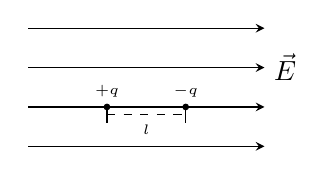
\begin{tikzpicture}
    \foreach \y in {0,0.5,1,1.5}
    \draw [->,>=stealth] (0,\y)--(3,\y); 
    \filldraw  (1,0.5) circle [radius=1pt] node [anchor=south] {\tiny $+q$};
    \filldraw  (2,0.5) circle [radius=1pt] node [anchor=south] {\tiny $-q$};
    \draw (1,0.5)--(1,0.3);
    \draw (2,0.5)--(2,0.3);
    \draw[dashed] (1,0.4)--(2,0.4);
    \draw (1.5,0.4) node [anchor=north]{\tiny $l$};
    \draw (3,1) node [anchor=west] {$\vec{E}$};
  \end{tikzpicture}
  \caption{电偶极子的极化能}
  \label{fig:dianoujizi}
\end{figure}

\begin{gather}
  \intertext{在图\ref{fig:dianoujizi}中所示电偶极子体系的电势能为}
  E_{pp}=q\varphi_+-q\varphi_-=-ql\frac{\varphi_+-\varphi_-}{l}
  \intertext{由电偶极子定义及电场强度计算公式可得上式为}
  E_p=-\vec{p}\cdot\vec{E}
  \intertext{如所考虑的区域存在多个电荷,则其总的能量可以表达为多个电偶极子能量之和,对上式的各电偶极子求和可得电极化强度$\vec{P}=\sum\vec{p}$,所以微小带电体系在静电场中所具有的电势能为}
  E_{pp}=-\vec{P}\cdot\vec{E}
\end{gather}

\subsection{磁化能}

考虑一个磁偶极子,一个矩形微小电流处于磁场中,如图\ref{fig:cioujizi}所示

\begin{figure}[H]
  \centering
  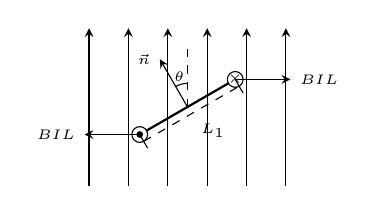
\begin{tikzpicture}
    \foreach \x in {-0.5,0,0.5,1,1.5,2}
    \draw [->,>=stealth] (\x,0)--(\x,2);
    \draw[thick] (0.75,1)++(210:0.6)--++(30:1.2);
    \draw (0.75,1)++(210:0.7) circle [radius=0.1]; 
    \filldraw (0.75,1)++(210:0.7) circle [radius=1pt]; 
    \draw (0.75,1)++(210:0.6)++(30:1.3) circle [radius=0.1];
    \draw (0.75,1)++(210:0.6)++(30:1.3) node {\tiny $\times$};
    \draw[->,>=stealth] (0.75,1)--++(120:0.7) node [anchor=east]{\tiny $\vec{n}$};
    \draw[->,>=stealth] (0.75,1)++(210:0.7)--++(180:0.7) node [anchor=east]{\tiny $BIL$}; 
    \draw[->,>=stealth] (0.75,1)++(210:0.6)++(30:1.3)--++(0:0.7) node [anchor=west]{\tiny $BIL$}; 
    \draw[dashed] (0.75,1)--(0.75,1.8);
    \draw(0.75,1.3) arc (90:120:0.3);
    \draw (0.75,1)++(105:0.4) node {\tiny $\theta$};
    \draw(0.75,1)++(210:0.7)--++(300:0.2);
    \draw(0.75,1)++(30:0.7)--++(300:0.2);
    \draw[dashed](0.75,1)++(210:0.7)++(300:0.1)--++(30:1.4);
    \draw(0.75,1)++(210:0.7)++(300:0.1)++(30:0.7) node [anchor=north west]{\tiny $L_1$};
  \end{tikzpicture}
  \caption{磁偶极子的能量}
  \label{fig:cioujizi}
\end{figure}

\begin{gather}
  \intertext{在图\ref{fig:cioujizi}中,磁偶极子垂直于纸面的宽度为$L$,在纸面上标出的部分长为$L_1$,求出其由图中所示角度转到$\theta=\frac{\pi}{2}$(零磁势能位置)安培力矩做功,则就是此位置时磁偶极子具备的磁化能,即}
  E_{pm}=\int_\theta^{\frac{\pi}{2}} BILL_1\sin\theta d\theta =-\vec{m}\cdot\vec{B}
  \intertext{由于电流分布区域非常小,所以可以视磁场为匀强磁场,同时将电流分解为若干个小环形电流,则求和可得此电流系统所具有的磁化能.磁化强度$\vec{M}=\sum\vec{m}$,所以得微小电流系统在磁场中所具有的磁化能为}
  E_{pm}=-\vec{M}\cdot\vec{B}
\end{gather}
\section{朗德因子}

这一节讨论在于说明统计物理学中关于理想气体磁性的相关公式,同时由于最初学习原子物理时,并没有接受自旋的概念,所以并不是很清楚朗德因子讨论的是什么问题.所以在读朗道的《统计力学》时,决定重新论证一下.

关于自旋,最初的感觉是不能接受,其原因在于平时学习时对于某些概念上理解的不足.但是伴随量子力学和电动力学的学习,我接受了这一概念,肯定这些基本粒子是有内部结构的或者是有自身运动则在以其质心为参考点的系统内,可以肯定其角动量的存在.但是朗道的观点我认为更加合理,当在球坐标系下描述粒子时,不是把粒子当成一个质点,它需要角部的描述,则必然存在一个$l$量子数,所以不必指明是什么来源也可以肯定其角动量的存在,所以自旋即是粒子的内禀角动量,所谓内禀角动量是指以其质心为参考系时,所计算出的角动量.\footnote{《朗道理论物理教程》\quad 卷一\quad 力学( 第5版) $\S 33$ 节.}

考虑到轨道角动量和自旋角动量的耦合,则轨道角动量就是粒子质心的运动所对应的角动量,而自旋是相对于质心坐标系的内禀角动量.但是当计算放在磁场中的带电系统时,其在磁场中的磁化能时所涉及的磁矩与角动量具备一定的关系,但不一定都是线性对应关系.

\begin{figure}[H]
  \centering
  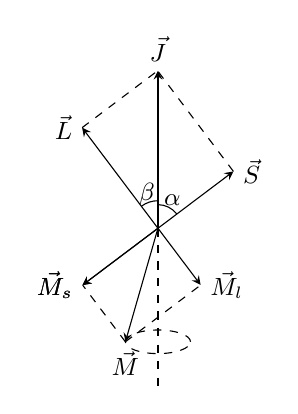
\begin{tikzpicture}
    \draw [->,>=stealth] (0,0)--(0,2) node [anchor=south] {\small $\vec{J}$}; 
    \draw [->,>=stealth] (0,0)--(37:1.2) node [anchor=west] {\small $\vec{S}$};
    \draw [->,>=stealth] (0,0)--(127:1.6) node [anchor=east] {\small $\vec{L}$};
    \draw [dashed] (37:1.2)--++(127:1.6);
    \draw [dashed] (127:1.6)--++(37:1.2);
    \draw [->,>=stealth] (0,0)--(217:1.2) node [anchor=east]{\small $\vec{M}_s$};
    \draw [->,>=stealth] (0,0)--(217:1.2) node [anchor=east]{\small $\vec{M}_s$};
    \draw [->,>=stealth] (0,0)--(307:0.9) node [anchor=west]{\small $\vec{M}_l$};
    \draw [->,>=stealth] (0,0)--(254:1.5) node [anchor=north]{\small $\vec{M}$};
    \draw [dashed] (254:1.5)--++(37:1.2);
    \draw [dashed] (254:1.5)--++(127:0.9);
    \draw [dashed] (0,0)--(0,-2);
    \draw (37:0.3) arc (37:90:0.3);
    \draw (63:0.4) node {\small $\alpha$};
    \draw (90:0.35) arc (90:127:0.35);
    \draw (108:0.45) node {\small $\beta$};
    \draw[dashed] (0,-1.4419) ellipse (0.4135 and 0.15);
  \end{tikzpicture}
  \caption{朗德因子的计算}
  \label{fig:langdeyinzi}
\end{figure}

\begin{gather}
  \intertext{一般情况下根据磁矩 $\vec{M}$ 和角动量$\vec{J}$ 的定义,可得轨道角动量 $\vec{L}$ 和轨道磁矩 $\vec{M}_l$ 的关系}
  \vec{M}_l=\frac{e}{2m}\vec{L}
  \intertext{考虑到量子表达式,则 Bohr 磁子(磁矩的自然单位)为$\mu$ $=$ $\frac{e\hbar}{2m}$, 则上式的标量式为}
  M_l =\mu\sqrt{l(l+1)}
  \intertext{在磁矩和角动量的关系中,质量$m$ 指的是运动粒子的净质量,但是电子的电磁质量和净质量不能明确区分开来,按照电动力学的结论可以取电磁质量和净质量相等,所以测得电子的质量就是这二者之和.因此对于电子内禀角动量自旋而言,则有关系}
  \vec{M}_s=\frac{e}{m}\vec{S}
  \intertext{则上式的标量式为}
  M_s =2\mu\sqrt{s(s+1)}
  \intertext{由于所研究的系统仅在磁场中时所受合外力矩为0,所以总角动量守恒,因此轨道角动量和自旋角动量所构成的平行四边形不变,但是还要绕总角动量方向转动,由于原子是稳定的,所以在所考虑的时间范围内轨道角动量和自旋角动量已经绕总角动量旋转了很多周,则总磁矩在总角动量垂直方向的分量在时间上平均值为零,因此整体上有效的磁矩是沿总角动量方向的分量$M_J$,即}
  \overline{M}=(L_J+2S_J)\frac{e}{2m}
  \label{eq:langde0}
  \intertext{据图\ref{fig:langdeyinzi},设各角动量的大小分别由其对应大写字母表示,对应量子数以其小写字母表示,则由勾股定理可得}
  \vec{L}^2+\vec{J}^2-\vec{S}^2=2\vec{L}\cdot\vec{J}
  \intertext{解得轨道角动量沿总角动量的分量$L_J$ 为}
  L_J=\frac{L^2+J^2-S^2}{2J}
  \intertext{对自旋角动量的沿总角动量的分量 $S_J$,同理可得}
  S_J=\frac{S^2+J^2-L^2}{2J}
  \intertext{代入式\eqref{eq:langde0}得}
  <\vec{M}> =\left\{
    1+\frac{j(j+1)-l(l+1)+s(s+1)}{2j(j+1)}
  \right\}\cdot\frac{e}{2m}\vec{J}
  \intertext{上式的标量式为}
  <M> =\left\{
    1+\frac{j(j+1)-l(l+1)+s(s+1)}{2j(j+1)}
  \right\}\cdot\sqrt{j(j+1)}\mu
  \intertext{记比例系数为$g$,此系数就是朗德因子,即}
  g=1+\frac{j(j+1)-l(l+1)+s(s+1)}{j(j+1)}
  \intertext{则此原子体系放入匀强磁场中的磁势能 $E_{pm}$ 为}
  E_{pm}=-\vec{M}\cdot\vec{B}
  \intertext{选外磁感应强度方向为$z$轴,所以记总角动量在$B$方向的投影为$m_j$,用系统总角动量表达上述磁势能,则}
  E_{pm}=g m_j \cdot \mu B \qquad (m_j=j,j-1,\cdots , -j+1,-j)
\end{gather}
